\section {Numerical Solution Technique}
\label{Num}

\subsection{Vertical and horizontal discretization}
\subsubsection{Horizontal grid}
\label{hori}
In the horizontal $(\xi,\eta)$, a traditional, centered, second-order
finite-difference approximation is adopted.  In particular, the
horizontal arrangement of variables is as shown in Fig.\ \ref{fcgr}.
This is equivalent to the well known Arakawa ``C'' grid, which is well
suited for problems with horizontal resolution that is fine compared to
the first radius of deformation (Arakawa and Lamb \cite{AL}).
\begin{figure}[htb]
\setlength{\unitlength}{6mm}
\thicklines
  \begin{picture}(19,12)(-8,0)
  \put(0,1.5){\line(1,0){12}}
  \put(0,8.5){\line(1,0){12}}
  \put(2,0){\line(0,1){10}}
  \put(10,0){\line(0,1){10}}
  \put(6,5){\circle{.4}}
\thinlines
  \put(6.5,9.6){\vector(1,0){3.5}}
  \put(5.5,9.6){\vector(-1,0){3.5}}
  \put(11.4,5.4){\vector(0,1){3.1}}
  \put(11.4,4.6){\vector(0,-1){3.1}}
  \put(1.5,5){\vector(1,0){1}}
  \put(9.5,5){\vector(1,0){1}}
  \put(6,1){\vector(0,1){1}}
  \put(6,8){\vector(0,1){1}}
  \put(6,9.6){\makebox(0,0){$\Delta\xi$}}
  \put(11.4,5){\makebox(0,0){$\Delta\eta$}}
  \put(6,5.4){\makebox(0,0)[b]{$(\rho,h,f,\Omega )_{i,j}$}}
  \put(1.8,5.3){\makebox(0,0)[br]{$u_{i,j}$}}
  \put(9.8,5.3){\makebox(0,0)[br]{$u_{i+1,j}$}}
  \put(5.8,1.3){\makebox(0,0)[tr]{$v_{i,j}$}}
  \put(5.8,8.3){\makebox(0,0)[tr]{$v_{i,j+1}$}}
  \end{picture}
\caption{Placement of variables on an Arakawa C grid}
\label{fcgr}
\end{figure}

\subsubsection{Vertical grid}
The vertical discretization also uses a second-order finite-difference
approximation.  Just as we use a staggered horizontal grid, the 
model was found to be more well-behaved with a staggered vertical
grid.  The vertical grid is shown in Fig.\ \ref{fvert}.

\begin{figure}[thb]
\setlength{\unitlength}{0.00083300in}%
%
\begin{picture}(987,2835)(-611,-3463)
\put(3166,-886){\circle*{120}}
\put(3166,-1336){\circle*{120}}
\put(3166,-1786){\circle*{120}}
\put(3166,-2236){\circle*{120}}
\put(3166,-2686){\circle*{120}}
\put(3166,-3136){\circle*{120}}
\put(2701,-661){\line( 1, 0){900}}
\put(3001,-1111){\line( 1, 0){300}}
\put(3001,-1561){\line( 1, 0){300}}
\put(3001,-2011){\line( 1, 0){300}}
\put(3001,-2461){\line( 1, 0){300}}
\put(3001,-2911){\line( 1, 0){300}}
\put(2701,-3361){\line( 1, 0){900}}
\put(3676,-736){\makebox(0,0)[lb]{$w_{\rm N}$}}
\put(3376,-961){\makebox(0,0)[lb]{$\rho_{\rm N}$}}
\put(3376,-3211){\makebox(0,0)[lb]{$\rho_1$}}
\put(3376,-2761){\makebox(0,0)[lb]{$\rho_2$}}
\put(3451,-2986){\makebox(0,0)[lb]{$w_1$}}
\put(3676,-3436){\makebox(0,0)[lb]{$w_0$}}
\put(3451,-2536){\makebox(0,0)[lb]{$w_2$}}
\put(3451,-1186){\makebox(0,0)[lb]{$w_{\rm N-1}$}}
\put(3376,-1411){\makebox(0,0)[lb]{$\rho_{\rm N-1}$}}
\end{picture}
\caption{Placement of variables on staggered vertical grid}
\label{fvert}
\end{figure}

\subsection{Masking of land areas}
\label{Mask1}
ROMS has the ability to work with interior land areas, although the
computations occur over the entire model domain.  One grid cell is
shown in Fig.\ \ref{fcgr} while several cells are shown in Fig.\
\ref{fmask1}, including two land cells.  The process of defining which
areas are to be masked is described in \S\ref{Mask}, while this
section describes how the masking affects the computation of the
various terms in the equations of motion.
\begin{figure}[t]
\setlength{\unitlength}{0.0125in}%
\begin{picture}(0,0)(-61,0)%
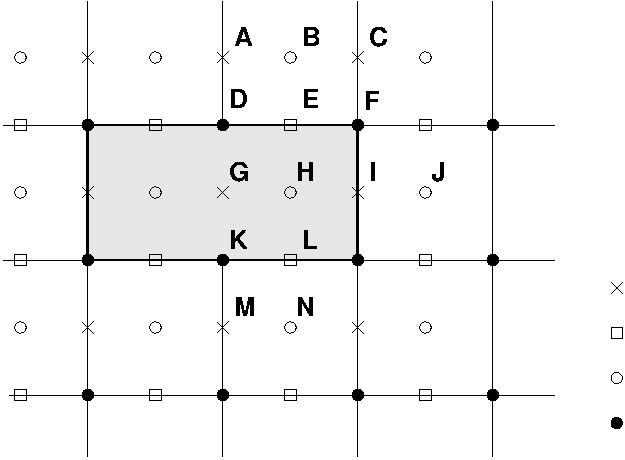
\includegraphics{pics/mask2}%
\end{picture}%
\begin{picture}(348,263)(92,465)
\put(490,552){\makebox(0,0)[lb]{-- $u$ points}}
\put(490,528){\makebox(0,0)[lb]{-- $v$ points}}
\put(490,504){\makebox(0,0)[lb]{-- $\rho$ points}}
\put(490,480){\makebox(0,0)[lb]{-- $\psi$ points}}
\end{picture}
\caption{Masked region within the domain}
\label{fmask1}
\end{figure}

\subsubsection{Velocity}
At the end of every time step, the values of many variables within the
masked region are set to zero by multiplying by the mask for either the
$u$, $v$ or $\rho$ points.  This is appropriate for the $v$ points {\bf
E} and {\bf L} in Fig.\ \ref{fmask1}, since the flow in and out of the
land should be zero.  It is likewise appropriate for the $u$ point at
{\bf I}, but is not necessarily correct for point {\bf G}.  The only
term in the $u$ equation that requires the $u$ value at point {\bf G}
is the horizontal viscosity, which has a term of the form
$\frac{\partial}{\partial \eta} \nu \frac{\partial u}{\partial \eta}$.
Since point {\bf G} is used in this term by both points {\bf A} and
{\bf M}, it is not sufficient to replace its value with that of the
image point for {\bf A}.  Instead, the term $\frac{\partial u}{\partial
\eta}$ is computed and the values at points {\bf D} and {\bf K} are
replaced with the values appropriate for either free-slip or no-slip
boundary conditions.  Likewise, the term $\frac{\partial}{\partial \xi}
\nu \frac{\partial v}{\partial \xi}$ in the $v$ equation must be corrected
at the mask boundaries.

This is accomplished by having a fourth mask array defined at the $\psi$
points, in which the values are set to be no-slip in \code{metrics}.
For no-slip boundaries, we count on the values inside
the land (point {\bf G}) having been zeroed out.  For point {\bf D}, the
image point at {\bf G} should contain minus the value of $u$ at point
{\bf A}.  The desired value of $\frac{\partial u}{\partial \eta}$ is
therefore $2 u_{\bf A}$ while instead we have simply $u_{\bf A}$.
In order to achieve the correct result, we multiply by a mask which
contains the value 2 at point {\bf D}.  It also contains a 2 at point
{\bf K} so that $\frac{\partial u}{\partial \eta}$ there will acquire
the desired value of $-2 u_{\bf M}$. The corner point {\bf F} is set to
have a value of 1.

\subsubsection{Temperature, salinity and surface elevation}

The handling of masks by the temperature, salinity and surface
elevation equations is similar to that in the momentum equations, and
is in fact simpler.  Values of $T$, $S$ and $\zeta$ inside the land
masks, such as point {\bf H} in Fig.\ \ref{fmask1}, are set to zero
after every time step.  This point would be used by the horizontal
diffusion term for points {\bf B}, {\bf J}, and {\bf N}.  This is
corrected by setting the first derivative terms at points {\bf E}, {\bf
I}, and {\bf L} to zero, to be consistent with a no-flux boundary
condition.
Note that the equation of state must be able to handle $T = S = 0$
since this is the value inside masked regions.

%\subsubsection{Free surface and pressure gradients}

%The surface elevation inside the land mask is simply used for setting
%the total depth and therefore the location of the $s$-coordinate
%surfaces.

\subsubsection{Wetting and drying}

There is now an option to have wetting and drying in the model, in
which a cell can switch between being wet or being dry as the tides
come in and go out, for instance. Cells which are masked out as in
Fig.~\ref{fmask1} are never allowed to be wet, however.
\begin{itemize}
   \item In the case of wetting and drying, a critical depth, $D_{crit}$,
is supplied by the user.
   \item The total water depth ($D=h+\zeta$) is compared to $D_{crit}$.
If the water level is less than this depth, no flux is allowed out
of that cell. Water can always flow in and resubmerge the cell.
  \item The wetting and drying only happens during the 2-D
computations; the 3-D computations see a depth of
$D_{crit}$ in the ``dry'' areas.
  \item The ice component now checks for dry cells when computing
the ice rheology.
\end{itemize}

\subsection{Time-stepping overview}

While time stepping the model, we have a stored history of the model fields
at time $n-1$, an estimate of the fields at the current time $n$, and
we need to come up with an estimate for time $n+1$. For reasons of
efficiency, we choose to use a split-explicit time step, integrating
the depth-integrated equations with a shorter time step than the full
3-D equations. There is an integer ratio $M$ between the time steps. The
exact details of how the time stepping is done vary from one version
of ROMS to the next, with the east coast ROMS described here being older
than other branches. Still, all versions have these steps:

\begin{enumerate}
  \item Take a predictor step for at least the 3-D tracers to time
  $n+\frac{1}{2}$.
  \item Compute $\overline{\rho}$ and
$\rho^*$ for use in the depth-integrated time steps, from the density
either at time $n$ or time $n+\frac{1}{2}$.
  \item Depth integrate the 3-D momentum right-hand side terms at
time $n+\frac{1}{2}$ for use in the depth-integrated time steps (or extrapolate
to obtain an estimate of those terms).
  \item Take all the depth-integrated steps. Store weighted
time-means of the $\overline{u}$, $\overline{v}$ fields centered at both
time $n+\frac{1}{2}$ and time $n+1$ (plus $\zeta$ at time $n+1$). The latter
requires this time stepping to extend past time $n+1$, using $M^*$ steps
rather than just $M$.
  \item Use the weighted time-means from depth-integrated fields to
complete the corrector step for the 3-D fields to time $n+1$.
\end{enumerate}
Great care is taken to avoid the introduction of a mode-splitting
instability due to the use of shorter time steps for the depth-integrated
computations.

The mode coupling has evolved through the various ROMS versions,
as shown in Fig.~\ref{ftimestep1} (from \cite{SS2008a}). The time stepping
schemes are also listed in Table~\ref{ttimestep1} and described in
detail in \cite{SS2005} and \cite{SS2008b}; the relevant ones
are described in Appendix~\ref{Frog}.

\begin{figure}[p]
\setlength{\unitlength}{1.0in}%
%
\begin{picture}(6.5,7.5)(0,0)
  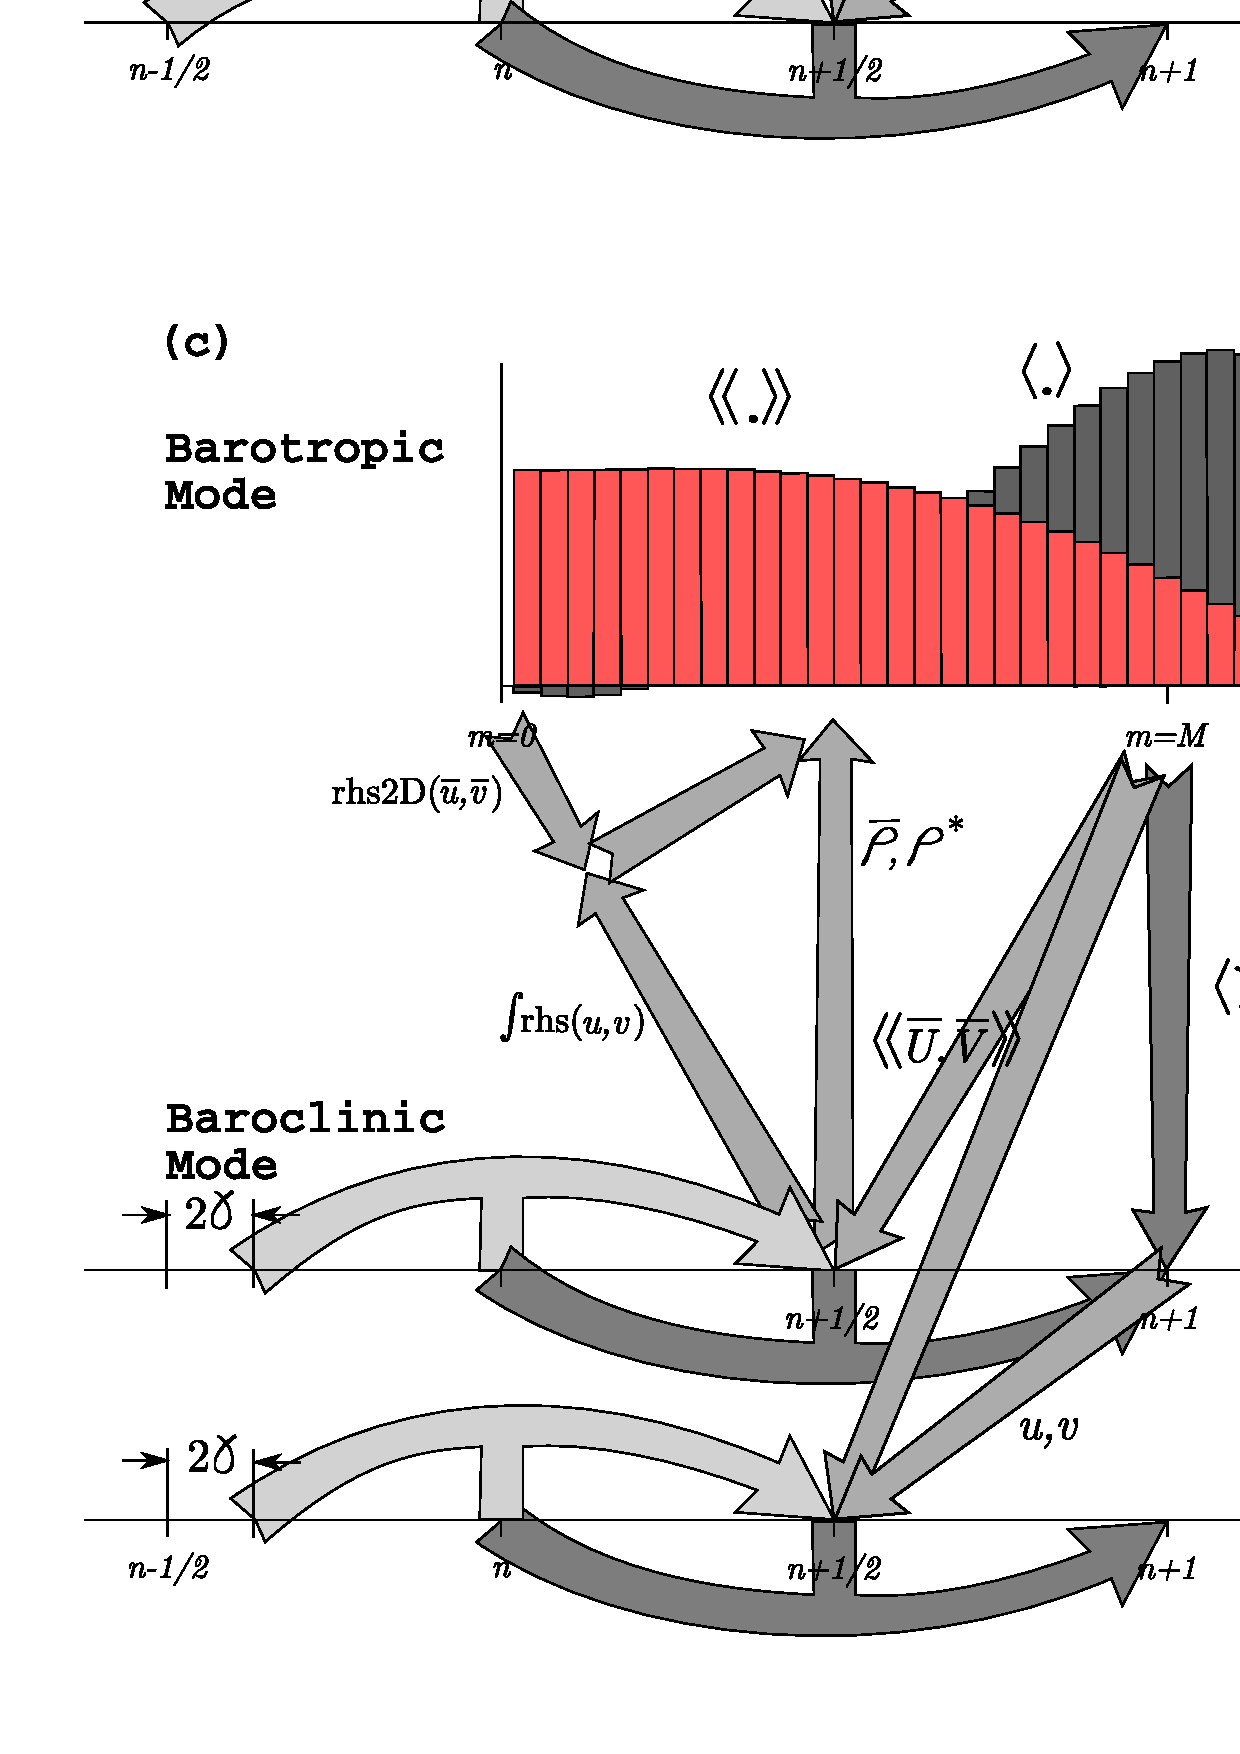
\includegraphics[width=6.5in]{pics/timestep_all}%
\end{picture}%
\caption{Diagrams of the time stepping and mode coupling used in
various ROMS versions. (a) Rutgers University ROMS (from
myroms.org), (b) ROMS AGRIF, (c) UCLA ROMS, described in \cite{SS2005},
(d) non-hydrostatic ROMS (\cite{Kanarska2007}). In all, the curved
arrows update the 3-D fields; those with ``pillars'' are leapfrog
in nature with the pillar representing the r.h.s. terms. Straight
arrows indicate exchange between the barotropic and baroclinic
modes. The shape functions for the fast time steps show just one
option out of many possibilities. The grey function has weights to
produce an estimate at time $n+1$, while the light red function has
weights to produce an estimate at time $n+\frac{1}{2}$.}
 \label{ftimestep1}
\end{figure}

\begin{table}[thb]
 \centerline{
\begin{tabular}{|l|c|c|c|c|c|} \hline
  & SCRUM 3.0 & Rutgers & AGRIF & UCLA & Non-hydrostatic \\
  \hline
  Reference & \cite{Hedstrom2000} & \cite{DAMEE_1} &
  \cite{Penven2006} & \cite{SS2005} & \cite{Kanarska2007} \\
  \hline
  Barotropic  & LF-TR & LF-AM3 with
  & LF-AM3 with & Gen. FB & Gen. FB \\
  mode & & FB feedback & FB feedback\footnote{The generalized FB
  barotropic mode was ported into the newest AGRIF code at the end
  of 2007.} & (AB3-AM4) & (AB3-AM4) \\
  \hline
  2-D $\alpha_{\max}$, iter. & $\sqrt{2}$,
  (2)\footnote{The number in parentheses (e.g., 2) indicates the
  number of r.h.s. computations per time step. If there are two
  parenthesized number, the first one is for momenta, the second for
  tracers.} & 1.85, (2) & 1.85,
  (2) & 1.78, (1) & 1.78, (1) \\
  \hline
  3-D momenta & AB3 & AB3 & LF-AM3 & LF-AM3 & AB3 (mod) \\
  \hline
  Tracers & AB3 & LF-TR & LF-AM3 & LF-AM3 & AB3 (mod) \\
  \hline
  Internal & AB3 & Gen.\ FB &
  LF-AM3, & LF-AM3, &
  Gen.\ FB \\
  waves & & (AB3-TR) & FB feedback & FB feedback & (AB3-AM4) \\
  \hline
  $\alpha_{\max}$, advect. & 0.72 & 0.72 & 1.587 &
  1.587 & 0.78 \\
  \hline
  $\alpha_{\max}$, Cor. & 0.72 & 0.72 & 1.587 &
  1.587 & 0.78 \\
  \hline
  $\alpha_{\max}$, int. w. & 0.72, (1) & 1.14,
  (1,2) & 1.85, (2) &
  1.85, (2) & 1.78, (1) \\
  \hline
  \end{tabular}
  }
\label{ttimestep1}
\caption{The time stepping schemes used in the various ROMS versions.
$\alpha \equiv \omega \delta t$ is the Courant number and $\omega=ck$
is the frequency for a wave component with wavenumber $k$.}
\end{table}

\subsection{Conservation properties}
\label{Enrg}
From Shchepetkin and McWilliams (2005) \cite{SS2005}, we have a
tracer concentration equation in advective form:
\begin{equation}
  \frac{\partial C}{\partial t} + (u \cdot \nabla) C = 0
  \label{eqt1}
\end{equation}
and also a tracer concentration equation in conservation form:
\begin{equation}
   \frac{\partial C}{\partial t} + \nabla \cdot (u C) = 0.
  \label{eqt2}
\end{equation}
The continuity equation:
\begin{equation}
   ( \nabla \cdot u) = 0
\end{equation}
can be used to get from one tracer equation to the other.
As a consequence of eq.~(\ref{eqt1}), if the tracer is spatially
uniform, it will remain so regardless of the velocity field
(constancy preservation). On the other hand, as a consequence of
(\ref{eqt2}), the volume integral of the tracer concentration is conserved
in the absence of internal sources and fluxes through the boundary. Both
properties are valuable and should be retained when constructing numerical
ocean models.

The semi-discrete form of the tracer equation
(\ref{st15}) is:
\begin{equation}
   \frac{\partial}{\partial t} \left( \frac{H_z C}{m n} \right)
   + \delta_{\xi} \left(
   \frac{u \overline{H_z}^\xi \overline{C}^\xi }{\overline{n}^\xi} \right)
   + \delta_{\eta} \left(
   \frac{v \overline{H_z}^\eta \overline{C}^\eta }{\overline{m}^\eta} \right)
   + \delta_\sigma \left( \overline{C}^\sigma
   \frac{H_z \Omega}{m n} \right) =
\\ \vspace{2mm}
   \frac{ 1}{mn} \frac{\partial}{\partial \sigma}
   \left( \frac{K_m}{\Delta z} \frac{\partial C}{\partial \sigma} \right) +
   {\cal D}_C + {\cal F}_C
\label{tfull}
\end{equation}
Here $\delta_{\xi}$, $\delta_{\eta}$ and $\delta_\sigma$ denote simple
centered finite-difference approximations to $\partial / \partial \xi$,
$\partial / \partial \eta$ and $\partial / \partial \sigma$ with the
differences taken over the distances $\Delta\xi$, $\Delta\eta$ and
$\Delta \sigma$, respectively. $\Delta z$ is the vertical distance from one
$\rho$ point to another. $\overline{ ( \hspace{5mm} )}^{\xi}$,
$\overline{ ( \hspace{5mm} )}^{\eta}$ and $\overline{ ( \hspace{5mm}
)}^\sigma$ represent averages taken over the distances $\Delta\xi$, $\Delta
\eta$ and $\Delta \sigma$. % $I_\sigma^0$ indicates a second-order vertical
%integral computed as a sum from level $\sigma$ to the surface at
%$\sigma=0$.

The finite volume version of the same equation is no different,
except that a quantity $C$ is defined as the volume-averaged
concentration over the grid box $\Delta V$:
\begin{equation}
   C = \frac{mn}{H_z} \int_{\Delta V} \frac{H_z C}{mn} \delta \xi
   \, \delta \eta \, \delta \sigma
\end{equation}
The quantity  $\left(
\frac{u \overline{H_z}^\xi \overline{C}^\xi}{\overline{n}^\xi} \right)$
is the flux through an interface between adjacent grid boxes.

This method of averaging was chosen because it internally conserves
first moments in the model domain, although it is still possible to
exchange mass and energy through the open boundaries. The method is
similar to that used in Arakawa and Lamb \cite{AL}; though their
scheme also conserves enstrophy. Instead, we will focus on (nearly) retaining
constancy preservation while coupling the barotropic
(depth-integrated) equations and the baroclinic equations.

The time step in eq.~(\ref{tfull}) is assumed to be from time $n$ to
time $n+1$, with the other terms being evaluated at time
$n+\frac{1}{2}$ for second-order accuracy.
Setting $C$ to 1 everywhere reduces eq.~(\ref{tfull}) to:
\begin{equation}
   \frac{\partial}{\partial t} \left( \frac{H_z}{m n} \right)
   + \delta_{\xi} \left(
   \frac{u \overline{H_z}^\xi }{\overline{n}^\xi} \right)
   + \delta_{\eta} \left(
   \frac{v \overline{H_z}^\eta}{\overline{m}^\eta} \right)
   + \delta_\sigma \left( 
   \frac{H_z \Omega}{m n} \right) = 0
\label{contfull}
\end{equation}
If this equation holds true for the step from time $n$ to time $n+1$, then
our constancy preservation will hold.

In a hydrostatic model such as ROMS, the discrete continuity
equation is needed to compute vertical velocity rather than grid-box
volume $\frac{H_z}{m n}$ (the latter is controlled by changes in
$\zeta$ in the barotropic mode computations). Here, $\frac{H_z
\Omega}{m n}$ is the finite-volume flux across the {\em moving}
grid-box interface, vertically on the $w$ grid.

The vertical integral of the continuity eq.~(\ref{st17}), using
the vertical boundary conditions on $\Omega$, is:
\begin{equation}
   \frac{\partial}{\partial t} \left( \frac{\zeta}{mn} \right) +
   \delta_{\xi} \left(
   \frac{\overline{u} \overline{D}^\xi }{\overline{n}^\xi} \right)
   + \delta_{\eta} \left(
   \frac{\overline{v} \overline{D}^\eta}{\overline{m}^\eta} \right)
   = 0
\label{zeta1}
\end{equation}
where $\zeta$ is the surface elevation, $D= h+\zeta$ is the total
depth, and $\overline{u},\overline{v}$ are the depth-integrated
horizontal velocities. This equation and the corresponding 2-D
momentum equations are time stepped on a shorter time step than 
eq.~(\ref{tfull}) and the other 3-D equations. Due to the details in
the mode coupling, it is only possible to maintain constancy
preservation to the accuracy of the barotropic time steps.

\subsection{Depth-integrated equations}
\label{Vort}
The depth average of a quantity $A$ is given by:
\begin{equation}
   \overline{A} = \frac{1}{D} \int_{-1}^0 H_z A d\sigma
\end{equation}
where the overbar indicates a vertically averaged quantity and
\begin{equation}
   D \equiv \zeta(\xi, \eta, t) + h(\xi, \eta)
\end{equation}
is the total depth of the water column.  The vertical integral of
equation (\ref{st13}) is:
%{\samepage
\begin{multline}
   \frac{\partial}{\partial t} \left( \frac{D \overline{u}}{mn} \right)
   + \frac 
   {\partial}{\partial \xi} \left( \frac{D \overline{uu}}{n} \right )
   + \frac 
   {\partial}{\partial \eta} \left( \frac{D \overline{uv}}{m} \right)
   - \frac{Df\overline{v}}{mn}
\\ \vspace{1mm}
   - \left[ \overline{vv}
   \frac{\partial}{\partial \xi}
   \left( \frac{1}{n} \right) - \overline{uv}
   \frac{\partial}{\partial \eta} \left(
   \frac{1}{m} \right) \right] D = 
   - \frac{D}{n}
   \left( \frac{\partial \overline{\phi_2}}{\partial \xi} +
   g \frac{\partial \zeta}{\partial \xi} \right)
\\ \vspace{1mm}
   + \frac{ D}{mn}
   \left( \overline{\cal F}_u + \overline{\cal D}_{h_u} \right) 
   + \frac{1}{mn} \left( \tau^{\xi}_s - \tau^{\xi}_b \right)
\label{ubar1}
\end{multline}
%}
where $\phi_2$ includes the $\frac{\partial z}{\partial \xi}$ term,
$\overline{\cal D}_{h_u}$ is the horizontal viscosity, and the
vertical viscosity only contributes through the upper and lower
boundary conditions.  The corresponding vertical integral of equation
(\ref{st14}) is:
%{\samepage
\begin{multline}
   \frac{\partial}{\partial t} \left( \frac{D \overline{v}}{mn} \right)
   + \frac 
   {\partial}{\partial \xi} \left( \frac{D \overline{uv}}{n} \right )
   + \frac 
   {\partial}{\partial \eta} \left( \frac{D \overline{vv}}{m} \right)
   + \frac{Df\overline{u}}{mn}
\\ \vspace{1mm}
   + \left[ \overline{uv}
   \frac{\partial}{\partial \xi}
   \left( \frac{1}{n} \right) - \overline{uu}
   \frac{\partial}{\partial \eta} \left(
   \frac{1}{m} \right) \right] D = 
   - \frac{D}{m}
   \left( \frac{\partial \overline{\phi_2}}{\partial \eta} +
   g \frac{\partial \zeta}{\partial \eta} \right)
\\ \vspace{1mm}
   + \frac{ D}{mn}
   \left( \overline{\cal F}_v + \overline{\cal D}_{h_v} \right) 
   + \frac{1}{mn} \left( \tau^{\eta}_s - \tau^{\eta}_b \right) .
\label{vbar1}
\end{multline}
%}
We also need the vertical integral of equation (\ref{st17}), shown
above as eq.~ (\ref{zeta1}).

The presence of a free surface introduces waves which propagate at a
speed of $\sqrt{gh}$.  These waves usually impose a more severe
time-step limit than any of the internal processes.  We have therefore
chosen to solve the full equations by means of a split time step.  In
other words, the depth integrated equations (\ref{ubar1}),
(\ref{vbar1}), and (\ref{zeta1}) are integrated using a short time step
and the values of $\overline{u}$ and $\overline{v}$ are used
to replace those found by integrating the full equations on a longer
time step.  A diagram of the barotropic time stepping is shown in
Fig.~\ref{ftspl}.
\begin{figure}[htb]
\setlength{\unitlength}{1.00in}%
%
\begin{picture}(5,2)(0,0.3)%
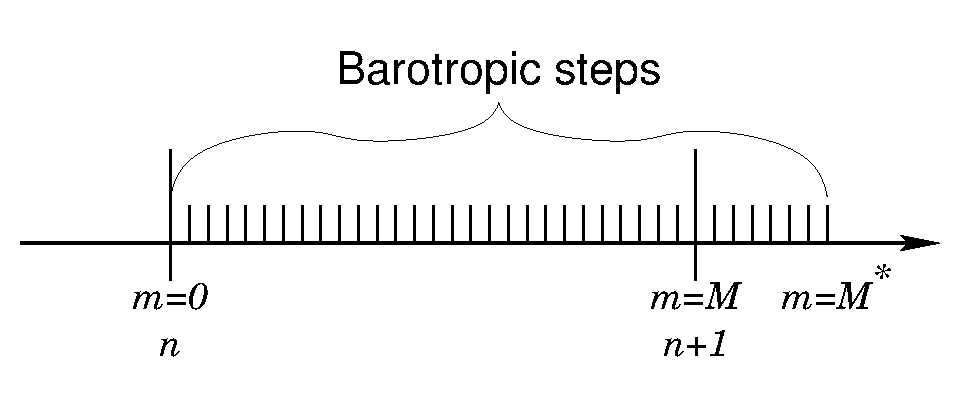
\includegraphics{pics/shortstep}%
\end{picture}%
 
 \caption{The split time stepping used in the model.}
 \label{ftspl}
\end{figure}

Some of the terms in equations (\ref{ubar1}) and (\ref{vbar1}) are
updated on the short time step while others are not.  The contributions
from the slow terms are computed once per long time step and stored.  If
we call these terms $R_{u_{\rm slow}}$ and $R_{v_{\rm slow}}$, equations
(\ref{ubar1}) and (\ref{vbar1}) become:
%{\samepage
\begin{multline}
   \frac{\partial}{\partial t} \left( \frac{D \overline{u}}{mn} \right)
   + \frac{\partial}{\partial \xi}
   \left( \frac{D \overline{u}\,\overline{u}}{n} \right)
   + \frac{\partial}{\partial \eta}
   \left( \frac{D \overline{u}\,\overline{v}}{m} \right)
   - \frac{Df\overline{v}}{mn}
\\ \vspace{1mm}
   - \left[ \overline{v}\,\overline{v}
   \frac{\partial}{\partial \xi}
   \left( \frac{1}{n} \right) - \overline{u}\,\overline{v}
   \frac{\partial}{\partial \eta} \left(
   \frac{1}{m} \right) \right] D = R_{u_{\rm slow}} -
   \frac{gD}{n} \frac{\partial \zeta}{\partial \xi}
    + \frac{D}{mn} {\cal D}_{\overline{u}}
   - \frac{1}{mn} \tau^{\xi}_b
\label{ubar2}
\end{multline}
%}  
%{\samepage
\begin{multline}
   \frac{\partial}{\partial t} \left( \frac{D \overline{v}}{mn} \right)
   + \frac{\partial}{\partial \xi}
   \left( \frac{D \overline{u}\,\overline{v}}{n} \right)
   + \frac{\partial}{\partial \eta}
   \left( \frac{D \overline{v}\,\overline{v}}{m} \right)
   + \frac{Df\overline{u}}{mn}
\\ \vspace{1mm}
   + \left[ \overline{u}\,\overline{v}
   \frac{\partial}{\partial \xi}
   \left( \frac{1}{n} \right) - \overline{u}\,\overline{u}
   \frac{\partial}{\partial \eta} \left(
   \frac{1}{m} \right) \right] D = R_{v_{\rm slow}} -
   \frac{gD}{m} \frac{\partial \zeta}{\partial \eta}
    + \frac{ D}{mn} {\cal D}_{\overline{v}}
   - \frac{1}{mn} \tau^{\eta}_b .
\label{vbar2}
\end{multline}
%}
When time stepping the model, we compute the right-hand-sides for
equations (\ref{st13}) and (\ref{st14}) as well as the
right-hand-sides for equations (\ref{ubar2}) and (\ref{vbar2}).  The
vertical integral of the 3-D right-hand-sides are obtained and then the
2-D right-hand-sides are subtracted.  The resulting fields are the slow
forcings $R_{u_{\rm slow}}$ and $R_{v_{\rm slow}}$.  This was found to
be the easiest way to retain the baroclinic contributions of the
non-linear terms such as $\overline{uu} - \overline{u}\,\overline{u}$.

The model is time stepped from time $n$ to time $n+1$ by using short
time steps on equations (\ref{ubar2}), (\ref{vbar2}) and (\ref{zeta1}).
Equation (\ref{zeta1}) is time stepped first, so that an estimate of the
new $D$ is available for the time rate of change terms
in equations (\ref{ubar2}) and (\ref{vbar2}).
A third-order predictor-corrector time stepping is used.
In practice, we actually time step all the way to time
$(n+\code{dtfast} \times M^\star)$,
while maintaining weighted averages of the values of $\overline{u}$,
$\overline{v}$ and $\zeta$.  The averages are used to replace the
values at time $n+1$ in both the baroclinic and barotropic modes,
and for recomputing the vertical grid spacing $H_z$.
Fig.~\ref{fbarostep1} shows one option for how these weights might look.

\begin{figure}[t]
\setlength{\unitlength}{1.in}%
\begin{picture}(6.5,7.5)(0,0)
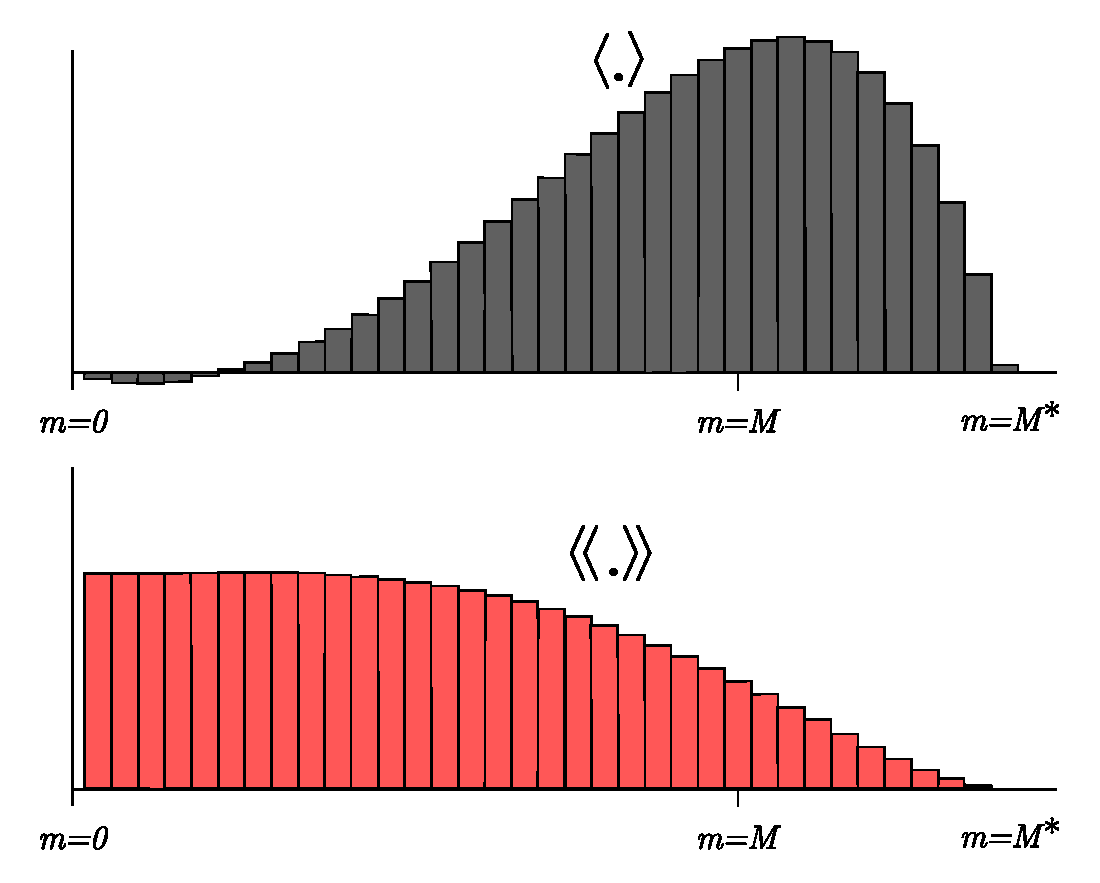
\includegraphics[width=6.5in]{pics/barostep}%
\end{picture}%
\caption{Weights for the barotropic time stepping. The upper panel
shows the primary weights, centered at time $n+1$, while the lower panel shows
the secondary weights weights, centered at time $n+\frac{1}{2}$.}
\label{fbarostep1}
\end{figure}

The primary weights, $a_m$, are used to compute $\langle \zeta
\rangle^{n+1} \equiv \sum_{m=1}^{M^\star} a_m \zeta^m$. There is a
related set of secondary weights $b_m$, used as $\langle \! \langle
\overline{u} \rangle \! \rangle^{n+\frac{1}{2}} \equiv \sum_{m=1}^{M^\star} b_m
\overline{u}^m$. In order to maintain constancy preservation, this
relation must hold:
\begin{equation}
  \langle \zeta \rangle_{i,j}^{n+1} = \langle \zeta \rangle_{i,j}^n -
  (mn)_{i,j} \Delta t \left[ \left\langle \!\! \left\langle
  \frac{D\overline u}{n} \right\rangle \!\!
  \right\rangle_{i+\frac{1}{2},j}^{n+\frac{1}{2}}
  - \left\langle \!\! \left\langle \frac{D\overline u}{n} \right\rangle
  \!\! \right\rangle_{i-\frac{1}{2},j}^{n+\frac{1}{2}} +
  \left\langle \!\! \left\langle
  \frac{D\overline v}{m} \right\rangle \!\!
  \right\rangle_{i,j+\frac{1}{2}}^{n+\frac{1}{2}}
  - \left\langle \!\! \left\langle \frac{D\overline v}{m} \right\rangle
  \!\! \right\rangle_{i,j-\frac{1}{2}}^{n+\frac{1}{2}} \right]
\label{zeta3}
\end{equation}
Shchepetkin and McWilliams (\cite{SS2005}) introduce a range of
possible weights, but the ones used here have a shape function:
\begin{equation}
   A(\tau) = A_0 \left\{ \left( \frac{\tau}{\tau_0} \right)^p \left[ 1-
   \left(\frac{\tau}{\tau_0} \right)^q \right] - r \frac{\tau}{\tau_0}
   \right\}
\label{weights}
\end{equation}
where $p, q$ are parameters and $A_0, \tau_0$, and $r$ are chosen to
satisfy normalization, consistency, and second-order accuracy
conditions,
\begin{equation}
   I_n = \int_0^{\tau^\star} \tau^n A(\tau) d \tau = 1, \quad n=0,1,2
\label{second}
\end{equation}
using Newton iterations. $\tau^\star$ is the upper limit of $\tau$
with $A(\tau) \geq 0$. In practice we initially set
$$
  A_0 = 1, r = 0 \mbox{and} \tau = \frac{(p+2)(p+q+2)}{(p+1)(p+q+1)}
$$
compute $A(\tau)$ using eq.~(\ref{weights}), normalize using:
\begin{equation}
   \sum_{m=1}^{M^\star} a_m \equiv 1, \quad
   \sum_{m=1}^{M^\star} a_m\frac{m}{M} \equiv 1,
\end{equation}
and adjust $r$ iteratively to satisfy the $n=2$ condition of
(\ref{second}). We are using values of $p=2$, $q=4$, and $r=0.284$.
This form allows some negative weights for small $m$, allowing
$M^\star$ to be less than $1.5M$.

ROMS also supports an older cosine weighting option, which isn't
recommended since it is only first-order accurate.

\subsection{Density in the mode coupling}

Equation (\ref{ubar2}) contains the term $R_{u_{\rm slow}}$,
computed as the difference between the 3-D right-hand-side and the
2-D right-hand-side. The pressure gradient therefore has the form:
\begin{equation}
   -\frac{g D}{n} \frac{\partial \zeta}{\partial \xi} +
   \left[\frac{g D}{n} \frac{\partial \zeta}{\partial \xi} + {\cal F}
   \right]
\end{equation}
where the term in square brackets is the mode coupling term and is
held fixed over all the barotropic steps and
\begin{equation}
  {\cal F} = - \frac{1}{\rho_0 n} \int_{-h}^\zeta \frac{\partial
  P}{\partial \xi} dz
\end{equation}
is the vertically integrated pressure gradient. The latter is a function
of the bathymetry, free surface gradient, and the free surface itself,
as well as the vertical distribution of density.

The disadvantage of this approach is that after the barotropic time
stepping is complete and the new free surface is substituted into
the full baroclinic pressure gradient, its vertical integral will
no longer be equal to the sum of the new surface slope term and the
original coupling term based on the old free surface. This is one
form of mode-splitting error which can lead to trouble because the
vertically integrated pressure gradient is not in balance with the
barotropic mass flux.

Instead, let us define the following:
\begin{equation}
  \overline{\rho} = \frac{1}{D} \int_{-h}^\zeta \rho dz , \quad
  \rho^\star = \frac{1}{\frac{1}{2} D^2} \int_{-h}^\zeta
  \left\{ \int_z^\zeta \rho dz^{\prime} \right\} dz
\end{equation}
Changing the vertical coordinate to $\sigma$ yields:
\begin{equation}
  \overline{\rho} =  \int_{-1}^0 \rho d\sigma , \quad
  \rho^\star = 2 \int_{-1}^0
  \left\{ \int_\sigma^0 \rho d\sigma^{\prime} \right\} d\sigma
\end{equation}
which implies that $\overline{\rho}$ and $\rho^\star$ are actually
independent of $\zeta$ as long as the density profile $\rho =
\rho(\sigma)$ does not change. The vertically integrated pressure
gradient becomes:
\begin{equation}
   -\frac{1}{\rho_0} \frac{g}{n} \left\{ \frac{\partial}{\partial \xi}
   \left( \frac{\rho^\star D^2}{2} \right) - \overline{\rho} D
   \frac{\partial h}{\partial \xi} \right\} = -\frac{1}{\rho_0}
   \frac{g}{n} D \left\{ \rho^\star \frac{\partial \zeta}{\partial \xi} +
   \frac{D}{2} \frac{\partial \rho^\star}{\partial \xi} + (\rho^\star -
   \overline{\rho}) \frac{\partial h}{\partial \xi} \right\}
\end{equation}
In the case of uniform density $\rho_0$, we obtain $\rho^\star \equiv
\overline{\rho} \equiv \rho_0$, but we otherwise have two new terms.
The accuracy of these terms depends on an accurate vertical
integration of the density, as described in Shchepetkin and
McWilliams (2005, \cite{SS2005}).

\subsection{Time stepping: internal velocity modes and tracers}
The momentum equations (\ref{st13}) and(\ref{st14}) are advanced before
the tracer equation, by computing all the terms except the vertical
viscosity and then using the implicit scheme described in \S\ref{Vfric}
to find the new values for $u$ and $v$. The depth-averaged component
is then removed and replaced by the $\langle \overline{u} \rangle$
and $\langle \overline{v} \rangle$ computed as in \S\ref{Vort}.
A third-order Adams-Bashforth (AB3) time stepping is used, requiring
multiple right-hand-side time levels (see Appendix~\ref{Frog}). These
stored up r.h.s. values can be used to extrapolate to a value at
time $n+\frac{1}{2}$ for use in the barotropic steps as shown in
Fig.~\ref{ftimestep1}.

The tracer concentration equation (\ref{tfull}) is advanced in a
predictor-corrector leapfrog-trapezoidal step, with great care taken to
optimize both the conservation and constancy-preserving properties of the
continuous equations. The corrector step can maintain both, as long as it
uses velocities and column depths which satisfy eq.~(\ref{zeta3}). This
also requires tracer values centered at time $n+\frac{1}{2}$, obtained
from the predictor step. The vertical diffusion is computed as in
\S\ref{Vfric}.

The predictor step cannot be both constancy-preserving and conservative; it
was therefore decided to make it constancy-preserving. Also, since it is
only being used to compute the advection for the corrector step, the
expensive diffusion operations are not carried out during the predictor step.

The preceeding notes on tracer advection refer to all but the MPDATA
option. The MPDATA algorithm has its own predictor-corrector with
emphasis on not allowing values to exceed their original range;
it therefore gives up the constancy-preservation. This is most
noticeable in shallow areas with large tides.

\subsection{Advection schemes}
\label{Advect}
Thus far, the advection scheme presented here is a centered
second-order scheme. This scheme is known to have some unfortunate
properties in the presence of strong gradients, such as large over- and
under-shoots of tracers, leading to the need for large amounts of
horizontal smoothing. SCRUM also provides two alternative advection
schemes with better behavior in many situations. At present, the
alternatives are only implemented in the full 3-D engine of the model.

\subsubsection{Third-order Upwind}
There is a class of third-order upwind advection schemes, both
one-dimensional (Leonard \cite{Leonard79}) and two-dimensional (Rasch
\cite{Rasch94}). This scheme is known as UTOPIA (Uniformly Third-Order
Polynomial Interpolation Algorithm). Applying flux limiters to UTOPIA
is explored in Thuburn \cite{Thuburn96}, although it is not implemented
in SCRUM. The two-dimensional formulation in Rasch contains terms of
order $u^2\psi$ and $u^3\psi$, including cross terms ($uv\psi$). The
terms which are nonlinear in velocity have been dropped in SCRUM,
leaving one extra upwind term in the computation of the advective
fluxes:
\begin{align}
   F^\xi &= \frac{H_z u}{n} \left( \psi - \gamma \frac{\partial^2
   \psi}{\partial \xi^2} \right) \\
   F^\eta &= \frac{H_z v}{m} \left( \psi - \gamma \frac{\partial^2
   \psi}{\partial \eta^2} \right)
\end{align}
The second derivative terms are centered on a $\rho$ point in the grid,
but are needed at a $u$ or $v$ point in the flux. The upstream value is
used [see equation (\ref{equp})]. The value of $\gamma$ in the model is
$\frac{1}{8}$ while that in Rasch \cite{Rasch94} is $\frac{1}{6}$.

Because the third-order upwind scheme is designed to be
two-dimensional, it is not used in the vertical (though one might argue
that we are simply performing one-dimensional operations here).
Instead, we use a centered fourth-order scheme in the vertical when
the third-order upwind option is turned on:
\begin{equation}
   F^s = \frac{H_z w}{mn} \left[
     - \frac{1}{16} \psi_{i,j,k-1} + \frac{9}{16} \psi_{i,j,k} +
       \frac{9}{16} \psi_{i,j,k+1} - \frac{1}{16} \psi_{i,j,k+2} \right]
\end{equation}

One advantage of UTOPIA over MPDATA is that it can be used on
variables having both negative and positive values. Therefore,
it can be used on velocity as well as scalars (is there a reference for
this?). For the $u$-velocity, we have:
\begin{align}
   F^\xi &= \left(u - \gamma \frac{\partial^2 u}{\partial \xi^2} \right)
   \left[ \frac{H_z u}{n} - \gamma \frac{\partial^2}{\partial \xi^2}
   \left( \frac{H_z u}{n} \right) \right] \\
   F^\eta &= \left(u - \gamma \frac{\partial^2 u}{\partial \eta^2}
     \right)
   \left[ \frac{H_z v}{m} - \gamma \frac{\partial^2}{\partial \xi^2}
   \left( \frac{H_z v}{m} \right) \right] \\
   F^\sigma &= \frac{H_z w}{mn} \left[
     - \frac{1}{16} u_{i,j,k-1} + \frac{9}{16} u_{i,j,k} +
       \frac{9}{16} u_{i,j,k+1} - \frac{1}{16} u_{i,j,k+2} \right]
\end{align}
while for the $v$-velocity we have:
\begin{align}
   F^\xi &= \left(v - \gamma \frac{\partial^2 v}{\partial \xi^2} \right)
   \left[ \frac{H_z u}{n} - \gamma \frac{\partial^2}{\partial \eta^2}
   \left( \frac{H_z u}{n} \right) \right] \\
   F^\eta &= \left(v - \gamma \frac{\partial^2 v}{\partial \eta^2}
     \right)
   \left[ \frac{H_z v}{m} - \gamma \frac{\partial^2}{\partial \eta^2}
   \left( \frac{H_z v}{m} \right) \right] \\
   F^\sigma &= \frac{H_z w}{mn} \left[
     - \frac{1}{16} v_{i,j,k-1} + \frac{9}{16} v_{i,j,k} +
       \frac{9}{16} v_{i,j,k+1} - \frac{1}{16} v_{i,j,k+2} \right]
\end{align}
In all these terms, the second derivatives are evaluated at an upstream
location.

\subsection{Determination of the vertical velocity and density fields}
\label{EOS}
Having obtained a complete specification of the $u,v,T,$ and $S$ fields
at the next time level by the methods outlined above, the vertical
velocity and density fields can be calculated.  The vertical velocity
is obtained by combining equations (\ref{st17}) and (\ref{zeta1}) to
obtain:
\begin{equation}
   \frac{\partial}{\partial \xi} \left( \frac{H_z u}{n} \right) +
   \frac{\partial}{\partial \eta} \left( \frac{H_z v}{m} \right) +
   \frac{\partial}{\partial \sigma}\left( \frac{H_z \Omega}{mn} \right)
   - \frac{\partial}{\partial \xi} \left( \frac{D \overline{u}}{n}
   \right) -
   \frac{\partial}{\partial \eta} \left( \frac{D \overline{v}}{m}
   \right)  = 0 .
\label{zeta2}
\end{equation}
Solving for $H_z \Omega / mn$ and using the semi-discrete notation of
\S\ref{Enrg} we obtain:
\begin{equation}
   \frac{H_z \Omega}{mn} =  \int  \left[
   \delta_{\xi} \left( \frac{\overline{u} \overline{D}^{\xi}}
   {\overline{n}^{\xi}} \right) +
   \delta_{\eta} \left( \frac{\overline{v} \overline{D}^{\eta}}
   {\overline{m}^{\eta}} \right) -
   \delta_{\xi} \left( \frac{u \overline{H_z}^{\xi}}
   {\overline{n}^{\xi}} \right) - 
   \delta_{\eta} \left( \frac{v \overline{H_z}^{\eta}}
   {\overline{m}^{\eta}} \right)  \right] d\sigma .
\label{omega}
\end{equation}
The integral is actually computed as a sum from the bottom upwards and
also as a sum from the top downwards.  The value used is a linear
combination of the two, weighted so that the surface down value is used
near the surface while the other is used near the bottom.

The density is obtained from temperature and salinity via an
equation of state.  SCRUM provides a choice of a nonlinear equation
of state $\rho = \rho(T,S,z)$ or a linear equation of state $\rho =
\rho(T)$.  The nonlinear equation of state has been modified and now
corresponds to the UNESCO equation of state as derived by Jackett and
McDougall \cite{Jackett}.  It computes {\sl in situ} density as a
function of potential temperature, salinity and pressure.

Warning: although we have used it quite extensively, McDougall
(personal communication) claims that the single-variable ($\rho =
\rho(T)$) equation of state is not dynamically appropriate as is.
He has worked out the extra source and sink terms required, arising
from vertical motions and the compressibility of water.  They are
quite complicated and we have not implemented them to see if they
alter the flow.

\subsection{The pressure gradient terms}
\label{PG}
The pressure gradient terms in equations (\ref{st13}) and
(\ref{st14}) are written in the form
\begin{equation}
  H_z \nabla \phi + \frac{g \rho H_z}{\rho_o} \nabla z
  + g H_z \nabla \zeta
\label{prgs}
\end{equation}
This is the form traditionally used in sigma-coordinate models to
account for the horizontal differences being taken along surfaces of
constant $\sigma$.  This form can be shown to lead to significant
errors when $|\nabla h|$ is large (Haney \cite{Haney}; and Beckmann
and Haidvogel \cite{BH93}). Shchepetkin....

\subsection{Open boundary conditions}
Need update for ROMS here...

\subsubsection{Gradient boundary condition}
This boundary condition is extremely simple and consists of setting the
gradient of a field to zero at the edge. The outside value is set equal
to the closest interior value. It is probably too simple to be useful
in realistic problems.

\subsubsection{Radiation boundary condition}
In realistic domains, open boundary conditions can be extremely
difficult to get right. There can be situations where incoming flow and
outgoing flow happen along the same boundary or even at the same
horizontal location. Orlanski \cite{Orlanski76} proposed a radiation
scheme in which a local phase velocity is computed and used to radiate
things out (if it is indeed going out). This works well for a wave
propagating normal to the boundary, but has problems when waves
approach the boundary at an angle. Raymond and Kuo \cite{Raymond84}
have modified the scheme to account for propagation in all three
directions. In SCRUM, only the two horizontal directions are accounted
for:
\begin{equation}
   \frac{\partial \psi}{\partial t} = - \left( C_x \frac{\partial
   \psi}{\partial \xi} + C_y \frac{\partial \psi}{\partial \eta}) \right)
\label{eqrk}
\end{equation}
where
\begin{align}
   C_x & = \frac{F \frac{\partial \psi}{\partial \xi}}{
   \left( \frac{\partial \psi}{\partial \xi} \right)^2 +
   \left( \frac{\partial \psi}{\partial \eta} \right)^2 } \\
   C_y & = \frac{F \frac{\partial \psi}{\partial \eta}}{
   \left( \frac{\partial \psi}{\partial \xi} \right)^2 +
   \left( \frac{\partial \psi}{\partial \eta} \right)^2 } \\
   F & = - \frac{\partial \psi}{\partial t}
\end{align}
These terms are evaluated at the closest interior point in a manner
consistent with the time stepping scheme used. The phase velocities are
limited so that the local CFL condition is satisfied. They are then
applied to the boundary point using equation (\ref{eqrk}), again using
a consistent time stepping scheme. Raymond and Kuo give the form used
for centered differencing and a leapfrog time step while SCRUM uses
one-sided differences.

The radiation approach is appropriate for waves leaving the domain. A
check is made to see which way the phase velocity is headed. If it is
entering the domain, a zero gradient condition is applied.
